\usepackage[utf8]{inputenc}
\usepackage[T1]{fontenc}
\usepackage[francais]{babel}
\usepackage{amsmath}
\usepackage{graphicx}
\usepackage{color}
\usepackage{pdfpages} 
\usepackage{listings}
\usepackage{graphicx}
\usepackage{hyperref}
\usepackage{amsthm}
\usepackage{amssymb}
\usepackage{mathrsfs}
\usepackage{moreverb}
\usepackage{titletoc}
\usepackage{lmodern}
\usepackage{cubeDrawing}
\usepackage{lipsum}
\usepackage{bbold}

\definecolor{oxf}{RGB}{0, 33, 71}
\definecolor{or}{RGB}{239, 155, 15}
\definecolor{vert}{RGB}{135,167,103}
\definecolor{rouge}{RGB}{181,39,39}
\definecolor{violet}{RGB}{64,9,90}


\newcommand{\oxf}[1]{\textcolor{oxf}{#1}}

%Macros pour modifier la table des matières
\hypersetup{colorlinks=true, urlcolor=bleu, linkcolor=black}
\usepackage{hyperref}

\titlecontents{chapter}[20pt]% 103
   {\addvspace{1pc}\normalfont\sffamily\bfseries\large} 
            {\contentslabel[\thecontentslabel]{20pt}}{}{\hfill\contentspage}[] 
\titlecontents{section}[40pt]% 
   {\addvspace{0.6pc}\normalfont\sffamily} 
            {\contentslabel[\thecontentslabel]{25pt}}{}{\dotfill\contentspage}[] 
\titlecontents{subsection}[60pt]% 
   {\addvspace{0.3pc}\normalfont\sffamily} 
            {\contentslabel[\thecontentslabel]{25pt}}{}{\dotfill\contentspage}[]                            
\titlecontents*{subsubsection}[60pt]% 
   {\filright\normalfont\sffamily\footnotesize}{}{}{}[~{–}\ ][] 
\setcounter{tocdepth}{2}

\makeatletter\@addtoreset{section}{part}
\makeatother



%Page de garde
\makeatletter

\def\graphic#1{\def\@graphic{#1}}
\graphic{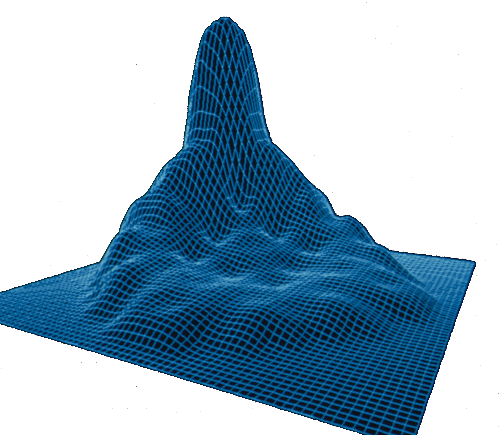
\includegraphics[scale=0.4]{logo.png}}
\def\clap#1{\hbox to 0pt{\hss #1\hss}}%
\def\ligne#1{%
\hbox to \hsize{%
\vbox{\centering #1}}}%
\def\haut#1#2#3{%
\hbox to \hsize{%
\rlap{\vtop{\raggedright #1}}%
\hss
\clap{\vtop{\centering #2}}%
\hss
\llap{\vtop{\raggedleft #3}}}}%
\def\bas#1#2#3{%
\hbox to \hsize{%
\rlap{\vbox{\raggedright #1}}%
\hss
\clap{\vbox{\centering #2}}%
\hss
\llap{\vbox{\raggedleft #3}}}}%
\def\maketitle{%
\thispagestyle{empty}\vbox to \vsize{%
\begin{tikzpicture}[remember picture,overlay]
\coordinate [below=2.5cm] (midpoint) at (current page.north);
\node [name=colourbar,
anchor=base,
fill=oxf,
minimum width=\paperwidth,
minimum height=1cm] at (midpoint){};
\node [
fill=oxf,
text = white,
xshift=2cm] at (midpoint){\Large{\textsf{Institut National des Sciences Appliquées de Rouen}}};
% Define the point where the logo will go
\coordinate [right=4cm] (logo) at (colourbar.west);
% Set coordinate system origin
\begin{scope}[shift=(logo)]
% Draw the outline
%\filldraw [white,draw=oxf] (2.3,0.85) -- (-2,0.85) -- (-2.8,-0.85) -- (2.3,-0.85) --cycle;
\filldraw [white,draw=oxf] (2.3,0.85) -- (-2.5,0.85) -- (-2.5,-0.85) -- (2.3,-0.85) --cycle;
\filldraw [oxf,draw=oxf] (-10,-24) -- (30,-24) -- (30,-23) -- (-10,-23) --cycle;
% Include the logo
\node {\includegraphics[width=4cm]{logoINSAdeRouen.jpg}};
\end{scope}
\end{tikzpicture}
\vspace{3cm}
%\usefont{OT1}{phv}{m}{n}
\begin{center}
\textbf{\huge \@title }
\end{center}
\vspace{1cm}
\par
\hrule height 4pt
\par
\vspace{0.5cm}
\begin{center}
\Large \@author
\par
\end{center}
\vfill
\begin{center}
\@graphic 
\end{center}
\vspace{1cm}
\haut{}{\@blurb}{}
\vspace{1cm}
\bas{}{\@date}{}
}
\cleardoublepage
}
\def\date#1{\def\@date{#1}}
\def\author#1{\def\@author{#1}}
\def\title#1{\def\@title{#1}}
\def\location#1{\def\@location{#1}}
\def\blurb#1{\def\@blurb{#1}}
\makeatother


\date{\today}
\title{Résolution numérique des équations de Saint-Venant par la méthode des éléments finis}
\author{Gabrielle Collette, Alexandre Vieira \& Conrad Hillairet}
\vfill
\blurb{
\textbf{Rapport}\\[1em]
Professeur référent : Christian Goût\\
}
